\section{Auswertung}
\label{sec:Auswertung}

Zur Auswertung wurden die Python-Bibliotheken \cite{numpy}, \cite{matplotlib} und \cite{uncertainties} genutzt.

\subsection{Messdaten}
\input{build/a_d.tex}

\begin{figure}
  \centering
  \begin{subfigure}{0.48\textwidth}
    \centering
    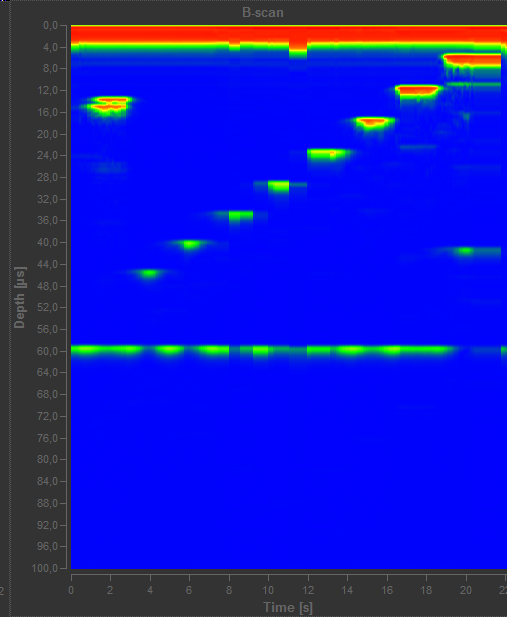
\includegraphics[width=\textwidth]{daten/b/1.png}
    \caption{Erster Scan, von oben.}
    \label{fig:db1}
  \end{subfigure}
  \begin{subfigure}{0.48\textwidth}
    \centering
    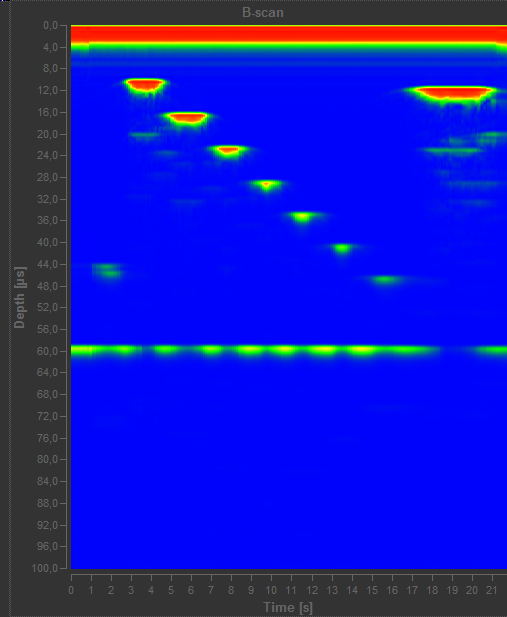
\includegraphics[width=\textwidth]{daten/b/2.png}
    \caption{Zweiter Scan, von unten.}
    \label{fig:db2}
  \end{subfigure}
  \caption{Originalbilder der B-Scans.}
  \label{fig:db}
\end{figure}
\fig{daten/tm/scan.png}{Originalbild des TM-Scans.}{dtm}[width=0.5\textwidth]
\FloatBarrier

\subsection{A-Scan}
Aus den gemessenen Zeiten können über Gl.~\eqref{eqn} die Tiefen $d_{1/2}$ ausgerechnet werden. Es wird eine Laufzeitkorrektur von
\begin{equation}
  t_\text{korr} = \SI{0.5}{µs},
\end{equation}
bedingt durch die Schutzschicht auf der Ultraschallsonde, abgezogen. Der Durchmesser der Störstellen $2r$ wird über
\begin{equation}
  2r = h - d_1 - d_2
\end{equation} mit der gemessenen Höhe
\begin{equation}
  h = \SI{80.04}{mm}
\end{equation}
des Acrylblocks berechnet. Dabei wird eine Schallgeschwindigkeit in Acryl von $\SI{2730}{\meter\per\second}$ \cite{olympus} angenommen. Die Ergebnisse, sowie die mit dem Messschieber gemessenen Längen finden sich in Tab.~\ref{tab:a}.
\begin{table}
        \caption{Messergebnisse aus dem A-Scan. Neben den abgelesenen und berechneten Daten $d_n$ sind auch die zuvor mittels Messschieber bestimmten Abmessungen $d_n^\text{mech}$ eingetragen.}
        \centering
        \label{tab:a}
        \begin{tabular}{l@{}S[round-mode=off, table-format=2.0]S[table-format=2.3, round-precision=4, round-mode=off] S[table-format=2.2, round-precision=4, round-mode=figures] S[table-format=1.4, round-precision=4, round-mode=figures] S[table-format=2.3, round-precision=4, round-mode=figures] S[table-format=2.2, round-precision=4, round-mode=figures] S[table-format=2.4, round-precision=4, round-mode=off] } \toprule & {$\text{Störstelle}$}& {$d_1/\si{mm}$}& {$d_2/\si{mm}$}& {$2r/\si{mm}$}& {$d_1^\text{mech}/\si{mm}$}& {$d_2^\text{mech}/\si{mm}$}& {$2r^\text{mech}/\si{mm}$}\\\midrule
& 1 & 18.02 & 61.56149999999999522515 & 0.46050000000000257394 & 19.62000000000000099476 & 59.61999999999999744205 & 0.80 \\
& 2 & 19.93 & 59.78699999999999192823 & 0.32400000000000828138 & 17.76000000000000156319 & 61.29999999999999715783 & 0.98 \\
& 3 & 61.29 & 13.78650000000000019895 & 4.96500000000000429878 & 61.28000000000000113687 & 13.43999999999999950262 & 5.32 \\
& 4 & 54.05 & 22.11299999999999599254 & 3.87300000000000821387 & 53.84000000000000341061 & 21.69999999999999928946 & 4.50 \\
& 5 & 46.68 & 30.43950000000000244427 & 2.91749999999998976818 & 46.50000000000000000000 & 30.07999999999999829470 & 3.46 \\
& 6 & 39.04 & 39.03900000000000147793 & 1.96199999999999152855 & 38.60000000000000142109 & 38.71999999999999886313 & 2.72 \\
& 7 & 31.12 & 47.09249999999999403144 & 1.82550000000000767209 & 30.82000000000000028422 & 46.88000000000000255795 & 2.34 \\
& 8 & 23.07 & 55.14600000000000079581 & 1.82550000000000411937 & 22.78000000000000113687 & 54.82000000000000028422 & 2.44 \\
& 9 & 15.01 & 62.92650000000001142553 & 2.09849999999999115019 & 14.82000000000000028422 & 62.97999999999999687361 & 2.24 \\
& 10 & 7.23 & 70.98000000000000397904 & 1.82549999999999990052 & 6.87999999999999989342 & 70.79999999999999715783 & 2.36 \\
& 11 & 55.82 & 15.42450000000000009948 & 8.78699999999999548095 & 55.11999999999999744205 & 14.63000000000000078160 & 10.29 \\
 \bottomrule \end{tabular} \end{table}


\subsection{B-Scan}
Die gleiche Messung wird erneut mit einem B-Scan durchgeführt und wie zuvor ausgewertet. Die Laufzeitkorrektur durch die Schutzschicht auf der Ultraschallsonde beträgt hier \begin{equation}
  t_\text{korr} = \SI{3.2}{µs},
\end{equation}
dies ist am gelben Balken im oberen Bereich der jeweiligen Diagramme zu erkennen.
Die grafischen Darstellungen der Scans finden sich in Abb.~\ref{fig:b1} und~\ref{fig:b2}. Daraus werden die in Tab.~\ref{tab:b} notierten Längen bestimmt.
\fig{build/b1.pdf}{Grafische Darstellung des ersten B-Scans (von oben), sowie der bestimmten Längen.}{b1}
\fig{build/b2.pdf}{Grafische Darstellung des zweiten B-Scans (von unten), sowie der bestimmten Längen. Störstelle 10 war in einer anderen Farbtabelle ablesbar (siehe Abb.~\ref{fig:b3}), die jedoch viel Rauschen erzeugte. Daher wurde die hier vorliegende Farbtabelle benutzt und nur der Messwert eingetragen.}{b2}
\fig{build/b3.pdf}{Variante von Abb.~\ref{fig:b2} mit veränderter Farbtabelle, Störstelle 10 ist deutlich zu erkennen.}{b3}
\begin{table}
        \caption{Messergebnisse aus dem B-Scan.}
        \centering
        \label{tab:b}
        \begin{tabular}{l@{}S[round-mode=off, table-format=2.0]S[table-format=2.3, round-precision=2, round-mode=places] S[table-format=2.2, round-precision=4, round-mode=figures] S[table-format=1.4, round-precision=4, round-mode=figures] S[table-format=2.3, round-precision=4, round-mode=figures] S[table-format=2.2, round-precision=4, round-mode=figures] S[table-format=2.4, round-precision=2, round-mode=places] } \toprule & {$\text{Störstelle}$}& {$d_1/\si{mm}$}& {$d_2/\si{mm}$}& {$2r/\si{mm}$}& {$d_1^\text{mech}/\si{mm}$}& {$d_2^\text{mech}/\si{mm}$}& {$2r^\text{mech}/\si{mm}$}\\\midrule& 1 & 19.79250000000000042633 & 60.05999999999999516831 & 0.18750000000000016653 & 19.62000000000000099476 & 59.61999999999999744205 & 0.80000000000000426326 \\
& 2 & 17.74500000000000099476 & 61.42499999999999005240 & 0.87000000000000965450 & 17.76000000000000156319 & 61.29999999999999715783 & 0.98000000000000397904 \\
& 3 & 61.42499999999999005240 & 13.64999999999999857891 & 4.96500000000000785150 & 61.28000000000000113687 & 13.43999999999999950262 & 5.32000000000000561329 \\
& 4 & 53.91749999999999687361 & 21.83999999999999985789 & 4.28250000000000152767 & 53.84000000000000341061 & 21.69999999999999928946 & 4.50000000000000355271 \\
& 5 & 46.40999999999999658939 & 30.02999999999999758415 & 3.60000000000000230926 & 46.50000000000000000000 & 30.07999999999999829470 & 3.46000000000000795808 \\
& 6 & 39.31199999999999761258 & 38.90249999999999630518 & 1.82550000000000078870 & 38.60000000000000142109 & 38.71999999999999886313 & 2.72000000000000596856 \\
& 7 & 30.71249999999999502620 & 47.09249999999999403144 & 2.23500000000000786926 & 30.82000000000000028422 & 46.88000000000000255795 & 2.34000000000000341061 \\
& 8 & 23.47799999999999798206 & 54.59999999999999431566 & 1.96200000000000551736 & 22.78000000000000113687 & 54.82000000000000028422 & 2.44000000000000483169 \\
& 9 & 15.01499999999999879208 & 62.78999999999999914735 & 2.23500000000000076383 & 14.82000000000000028422 & 62.97999999999999687361 & 2.24000000000000198952 \\
& 10 & 7.09799999999999986500 & 71.66249999999999431566 & 1.27950000000001673506 & 6.87999999999999989342 & 70.79999999999999715783 & 2.36000000000001364242 \\
& 11 & 55.96500000000000341061 & 15.01499999999999879208 & 9.06000000000000049738 & 55.11999999999999744205 & 14.63000000000000078160 & 10.29000000000000802913 \\
 \bottomrule \end{tabular} \end{table}


\subsection{TM-Scan}
Zuletzt wird das Herzmodell, beschrieben in Abschnitt~\ref{sec:durchführung}, untersucht. Der TM-Scan ist in Abb.~\ref{fig:tm1} und~\ref{fig:tm2}, die daraus gewonnen Daten in Tab.~\ref{tab:tm} zu finden. Die gemittelte Herzfrequenz ist
\begin{equation}
  \nu_\text{Herz} = \SI{0.652+-0.007}{\hertz} = \SI{39.1+-0.4}{\per\minute}.
\end{equation}
Für die Schallgeschwindigkeit in Wasser wird hier
\begin{equation}
  c = \SI{1480}{\meter\per\second},
\end{equation}
ebenfalls aus \cite{olympus}, angenommen.
Die zuerst durchgeführte Messung des Tiefenunterschieds zwischen ungepumptem und gepumptem Zustand im Herzmodell mit einem A-Scan ergibt
\begin{align*}
  t_\text{A-Scan}^\text{ESV} &= \SI{48.4}{µs} \\
  t_\text{A-Scan}^\text{EDV} &= \SI{16.2}{µs} \\
  \intertext {und demnach}
  \Delta t_\text{A-Scan} &= \SI{48.4}{µs} - \SI{16.2}{µs} = \SI{32.2}{µs}, \\
  \intertext {woraus wiederum aus Gleichung \eqref{eqn}}
  \Delta d_\text{A-Scan} &= \SI{2.38}{cm}
\end{align*}
gefolgert werden kann.
Im TM-Scan wurden für die enddiastolische Messtiefe mehrere Messwerte gemittelt, die Einzelwerte sind in Abb.~\ref{fig:tm1} und Tab.~\ref{tab:tm} zu erkennen.
Es folgt
\begin{align*}
  \Delta t_\text{TM-Scan} &= \SI{44}{µs} - \SI{2.81+-0.08}{µs}, \\
  \intertext{dann erneut über Gleichung \eqref{eqn}}
  \Delta d_\text{TM-Scan} &= \SI{3.048+-0.006}{cm}.
\end{align*}
Daraus folgt über das Volumen eines Kugelsegments (\cite{wurst}) das Schlagvolumen
\begin{equation}
  SV = \frac{1}{3} \pi (\Delta d)^2 (3R - \Delta d)
\end{equation}
für die jeweiligen Messreihen ergibt sich daraus
\begin{align*}
  SV_\text{A-Scan} &= \SI{67.17}{\cubic\centi\meter} \\
  SV_\text{TM-Scan} &= \SI{103.43+-0.35}{\cubic\centi\meter}
\end{align*}
und über
\begin{equation}
  HZV = SV \cdot \nu_\text{Herz}
\end{equation}
das Herzzeitvolumen
\begin{align*}
  HZV_\text{A-Scan} &= \SI{43.8+-0.5}{\cubic\centi\meter\per\second} \\
  HZV_\text{TM-Scan} &= \SI{67.5+-0.7}{\cubic\centi\meter\per\second}.
\end{align*}
\begin{table}
        \caption{Messergebnisse des Herzmodells. $t$ beschreibt dabei den Zeitpunkt des Herzschlags und $d$ die enddiastolische Messtiefe.}
        \centering
        \label{tab:tm}
        \begin{tabular}{l@{}S[table-format=2.1, round-precision=1, round-mode=places] S[table-format=1.1, round-precision=1, round-mode=places] |S[table-format=2.1, round-precision=1, round-mode=places] S[table-format=1.1, round-precision=1, round-mode=places] } \toprule & {$t/\si{s}$}& {$d/\si{µs}$}& {$t/\si{s}$}& {$d/\si{µs}$}\\\midrule& 1.19999999999999995559 & 2.00000000000000000000 & 13.40000000000000035527 & 2.79999999999999982236 \\
& 2.70000000000000017764 & 2.50000000000000000000 & 15.00000000000000000000 & 2.70000000000000017764 \\
& 4.20000000000000017764 & 2.70000000000000017764 & 16.50000000000000000000 & 3.10000000000000008882 \\
& 5.79999999999999982236 & 3.00000000000000000000 & 18.00000000000000000000 & 3.10000000000000008882 \\
& 7.29999999999999982236 & 3.00000000000000000000 & 19.60000000000000142109 & 2.29999999999999982236 \\
& 8.69999999999999928946 & 3.10000000000000008882 & 21.10000000000000142109 & 2.70000000000000017764 \\
& 10.19999999999999928946 & 3.20000000000000017764 & 22.69999999999999928946 & 2.89999999999999991118 \\
& 11.80000000000000071054 & 3.00000000000000000000 & 24.19999999999999928946 & 2.89999999999999991118 \\
 \bottomrule \end{tabular} \end{table}

\fig{build/tm.pdf}{Time-Motion-Scan des Herzmodells.}{tm1}
\fig{build/tm_zoom.pdf}{Kleinerer Zeitausschnitt aus dem Time-Motion-Scan.}{tm2}
